\makeatletter
\def\input@path{{../../tex/}{../another-directory/}}
\makeatother

\documentclass[aspectratio=169]{beamer}

% Document metadata
\title{ExaMA}
\subtitle{Methods and Algorithms at ExaScale}
\author[CP/HB]{Christophe Prud'homme \& Hélène Barucq}
\institute{}
\date{\today}

% Image for the title page (use includegraphics option to properly size/place it)
\titlegraphic{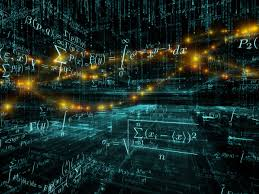
\includegraphics[height=\paperheight]{../../figures/math-hpc.jpeg}}

\usetheme[sectionstyle=style2]{trigon}

% Define logos to use (comment if no logo)
\biglogo{../../figures/exascale.png} % Used on titlepage only
\smalllogo{../../figures/exascale.png} % Used on top right corner of regular frames

% ------ If you want to change the theme default colors, do it here ------
%\definecolor{tPrim}{HTML}{00843B}   % Green
%\definecolor{tSec}{HTML}{289B38}    % Green light
%\definecolor{tAccent}{HTML}{F07F3C} % Orange

% ------ Packages and definitions used for this demo. Can be removed ------
\usepackage{appendixnumberbeamer} % To use \appendix command
\pdfstringdefDisableCommands{% Fix hyperref translate warning with \appendix
\def\translate#1{#1}%
}
\usepackage{pgf-pie} % For pie charts
\usepackage{caption} % For subfigures
\usepackage{subcaption} % For subfigures
\usepackage{xspace}
\newcommand{\themename}{\textbf{\textsc{trigon}}\xspace}
\usepackage[scale=2]{ccicons} % Icons for CC-BY-SA
\usepackage{booktabs} % Better tables

%==============================================================================
%                               BEGIN DOCUMENT
%==============================================================================
\begin{document}

\section{Project planning}
\begin{frame}
  \frametitle{\insertsectionhead}
  \framesubtitle{\insertsubsectionhead}
  \begin{itemize}
      \item Create issues(tasks), 
      \item break them into tasks, 
      \item track relationships, 
      \item add/use custom fields, 
      \item and have conversations. 
  \end{itemize}
  \alert{Visualize large projects as spreadsheets or boards, and automate everything with code.}
\end{frame}
\section{Table vs Board Views}
\begin{frame}
  \frametitle{\insertsectionhead}
  \framesubtitle{\insertsubsectionhead}
  \begin{columns}{T}
    \column{.45\textwidth}
    \begin{itemize}
        \item Built like a spreadsheet, project tables give a live workspace to filter, sort, and group issues and pull requests. 
        \item We can tailor them to your needs with custom fields and saved views.
        \item boards can display group issues using custom fields (e.g. Status)
    \end{itemize}
    \column{.5\textwidth}
    \only<1>{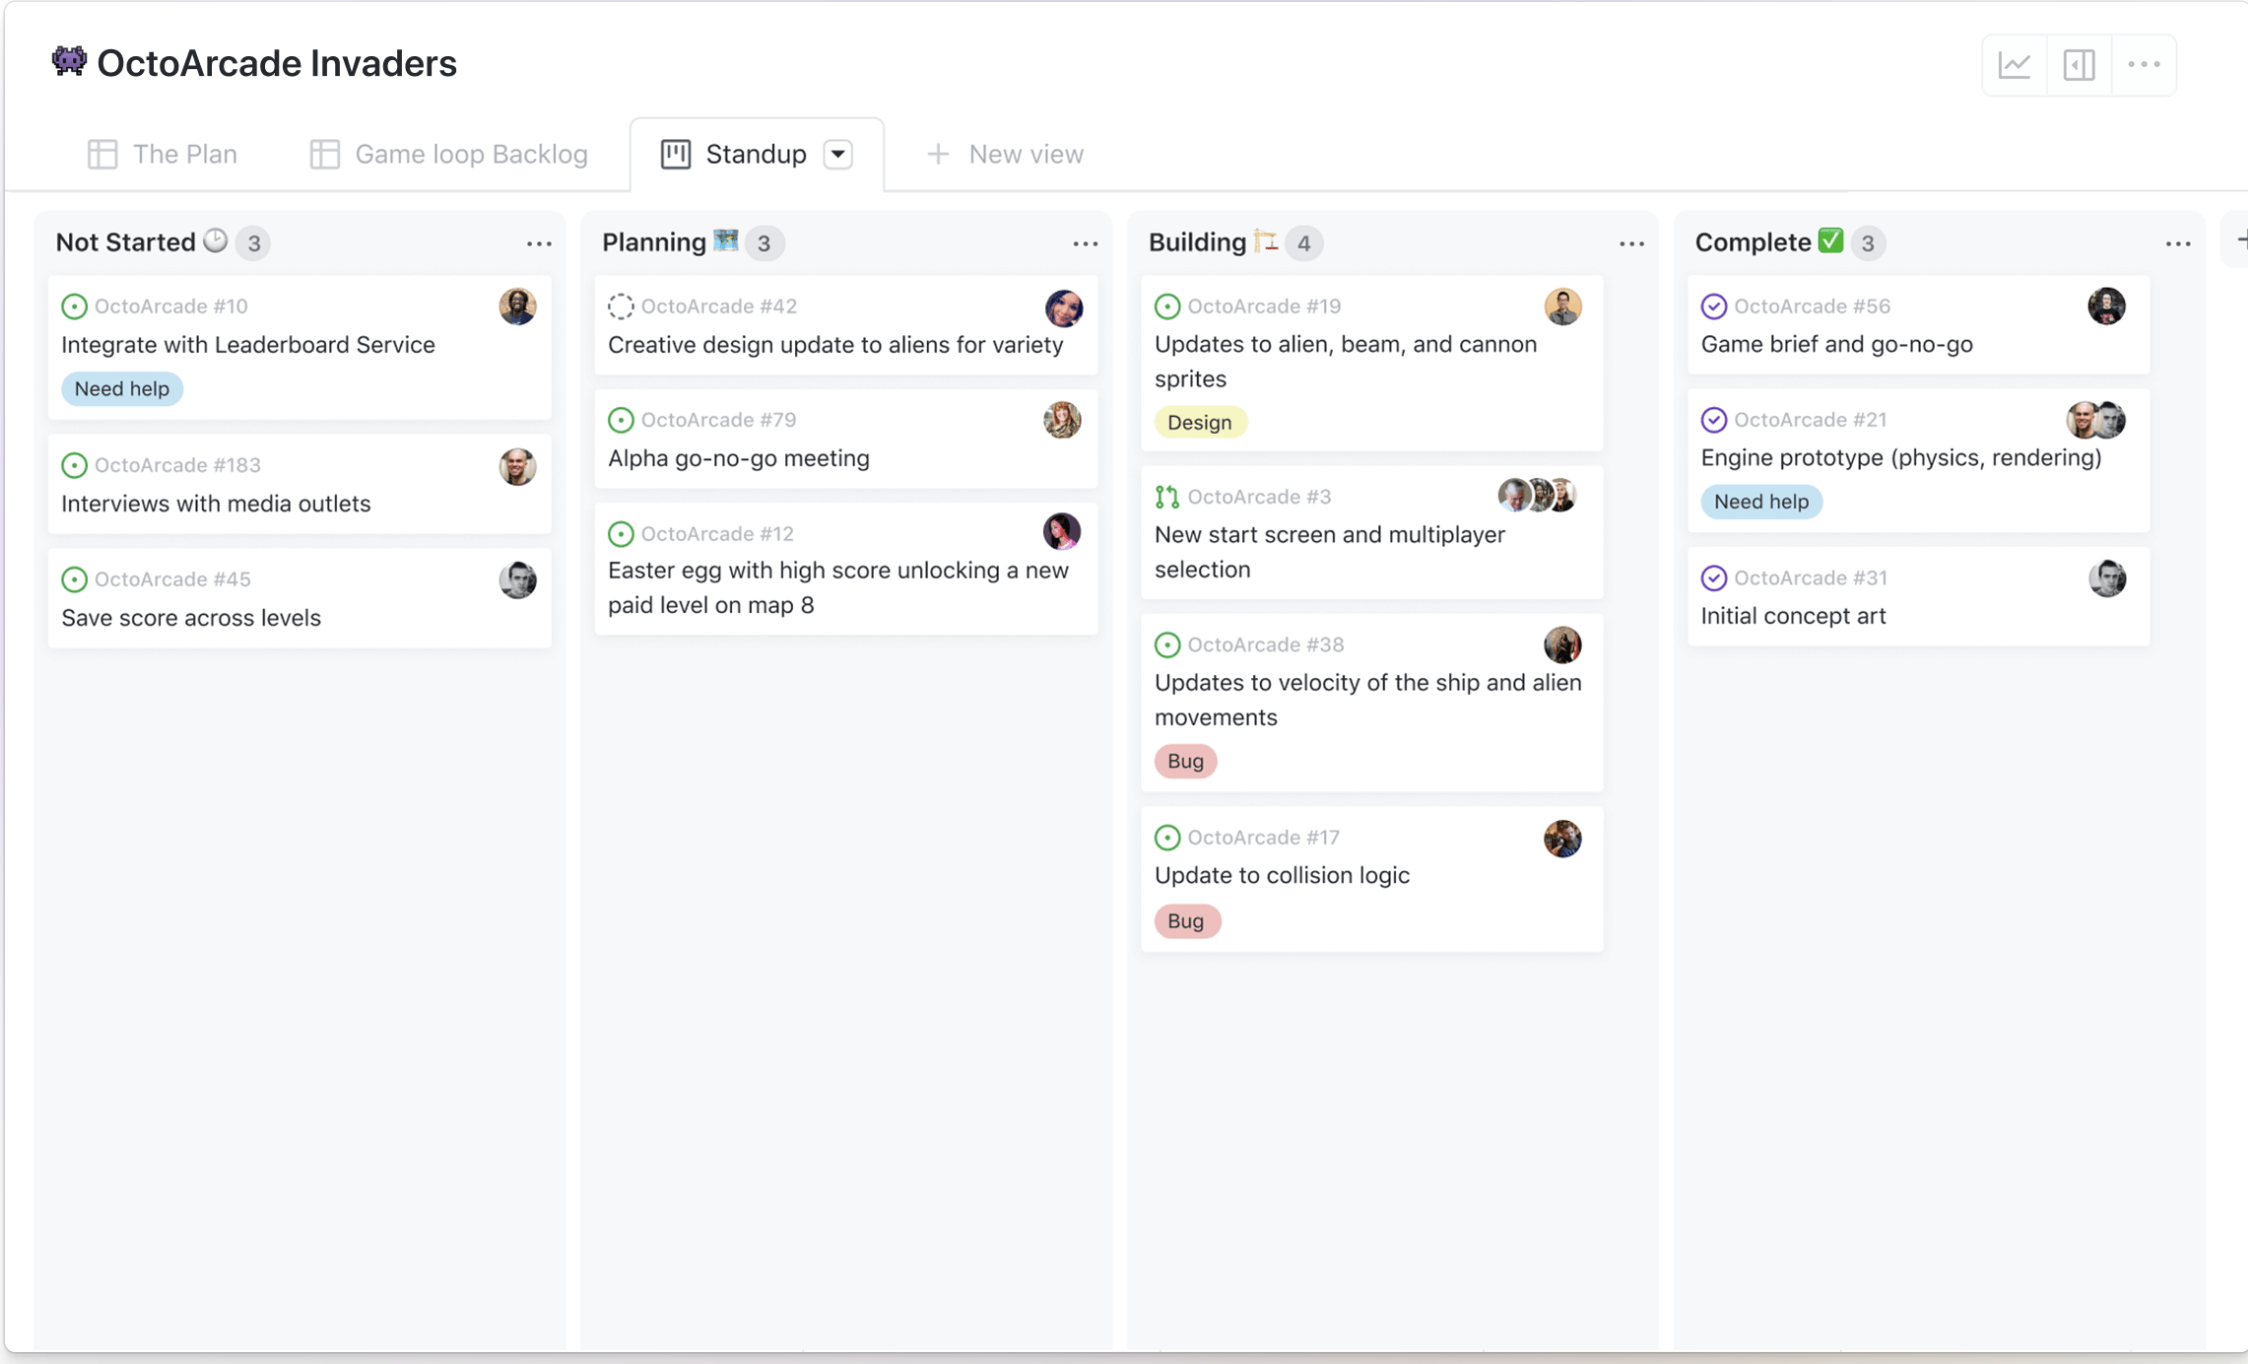
\includegraphics[width=.9\linewidth]{../../figures/board-view.png}}
    \only<2>{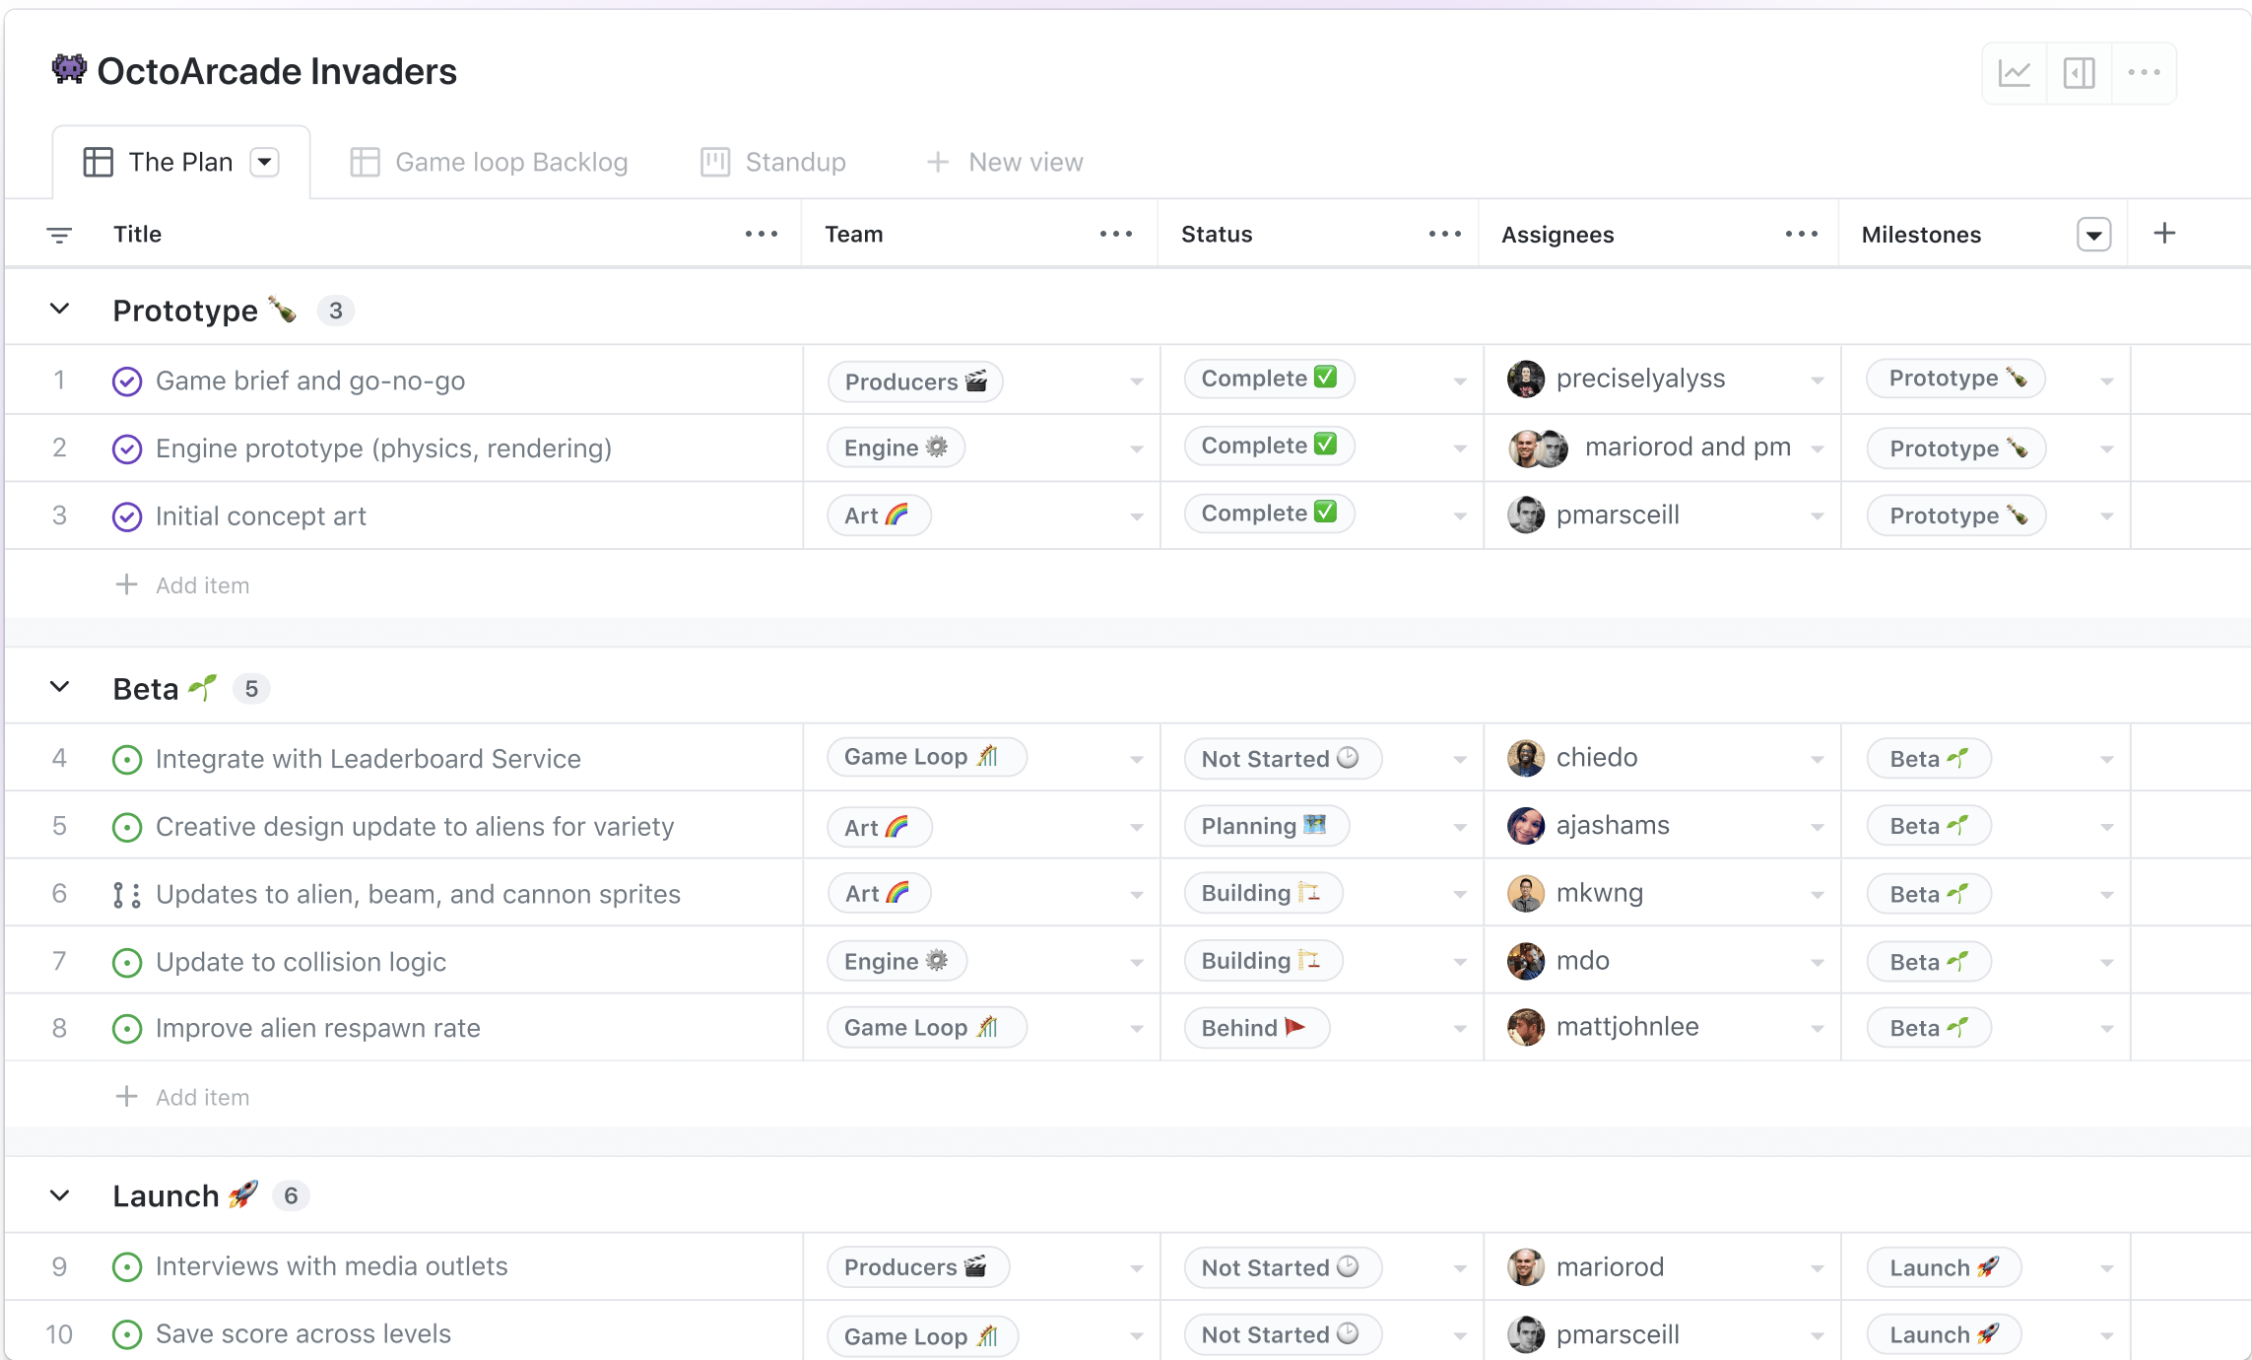
\includegraphics[width=.9\linewidth]{../../figures/table-view.png}}
  \end{columns}
\end{frame}

\section{Break issues into actionable tasks}

\begin{frame}
  \frametitle{\insertsectionhead}
  \framesubtitle{\insertsubsectionhead}
  \begin{columns}
    \column{.45\textwidth}
    \begin{itemize}
      \item Tackle complex issues with task lists 
      \item track their status with new progress indicators. 
      \item Convert tasks into their own issues 
      \item navigate your work hierarchy.
  \end{itemize}
  \column{.5\textwidth}
    \only<1>{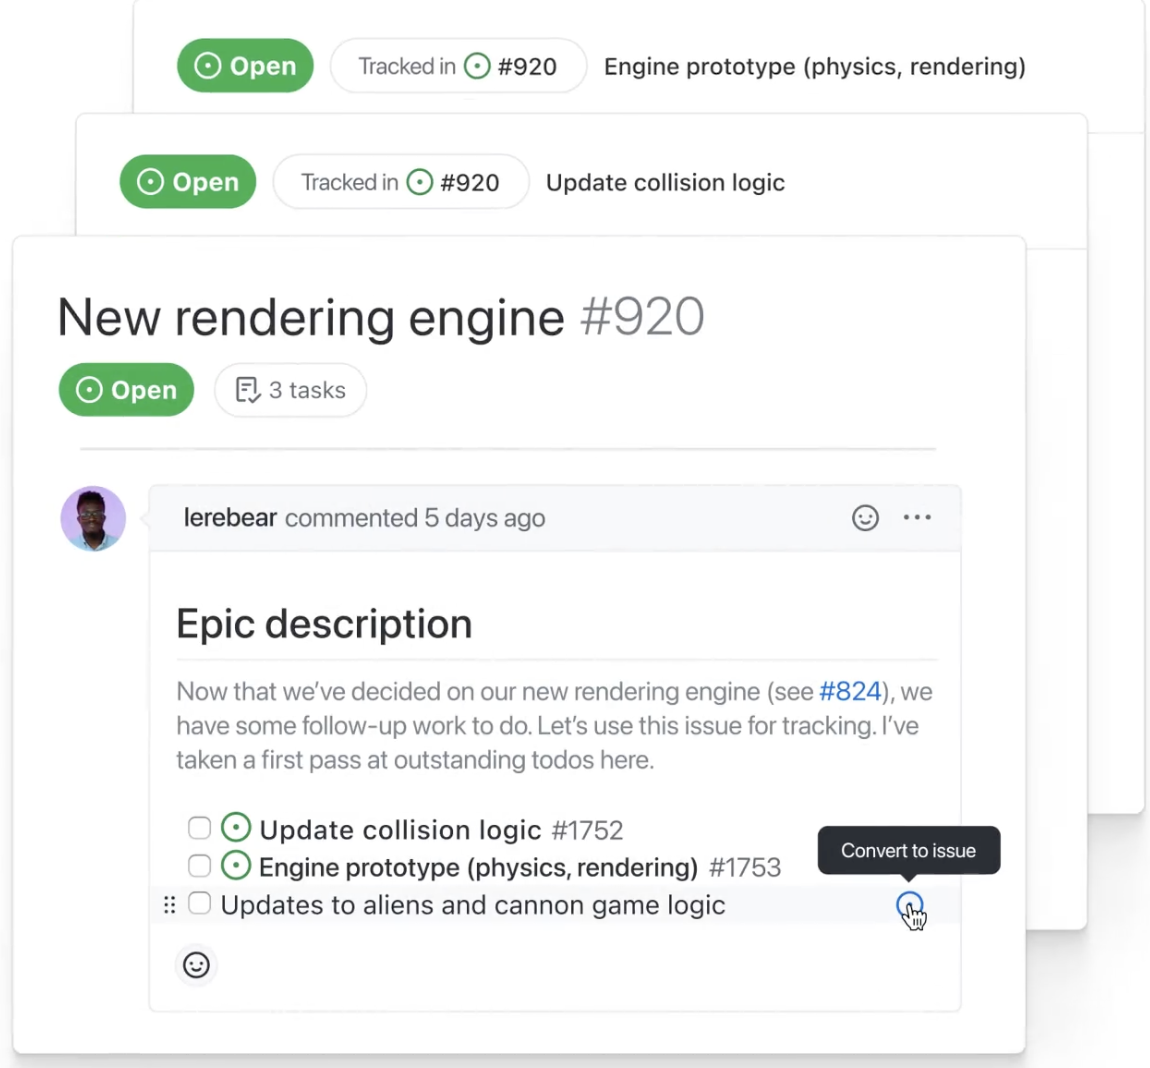
\includegraphics[width=.9\linewidth]{../../figures/issues-1.png}}
    \only<2>{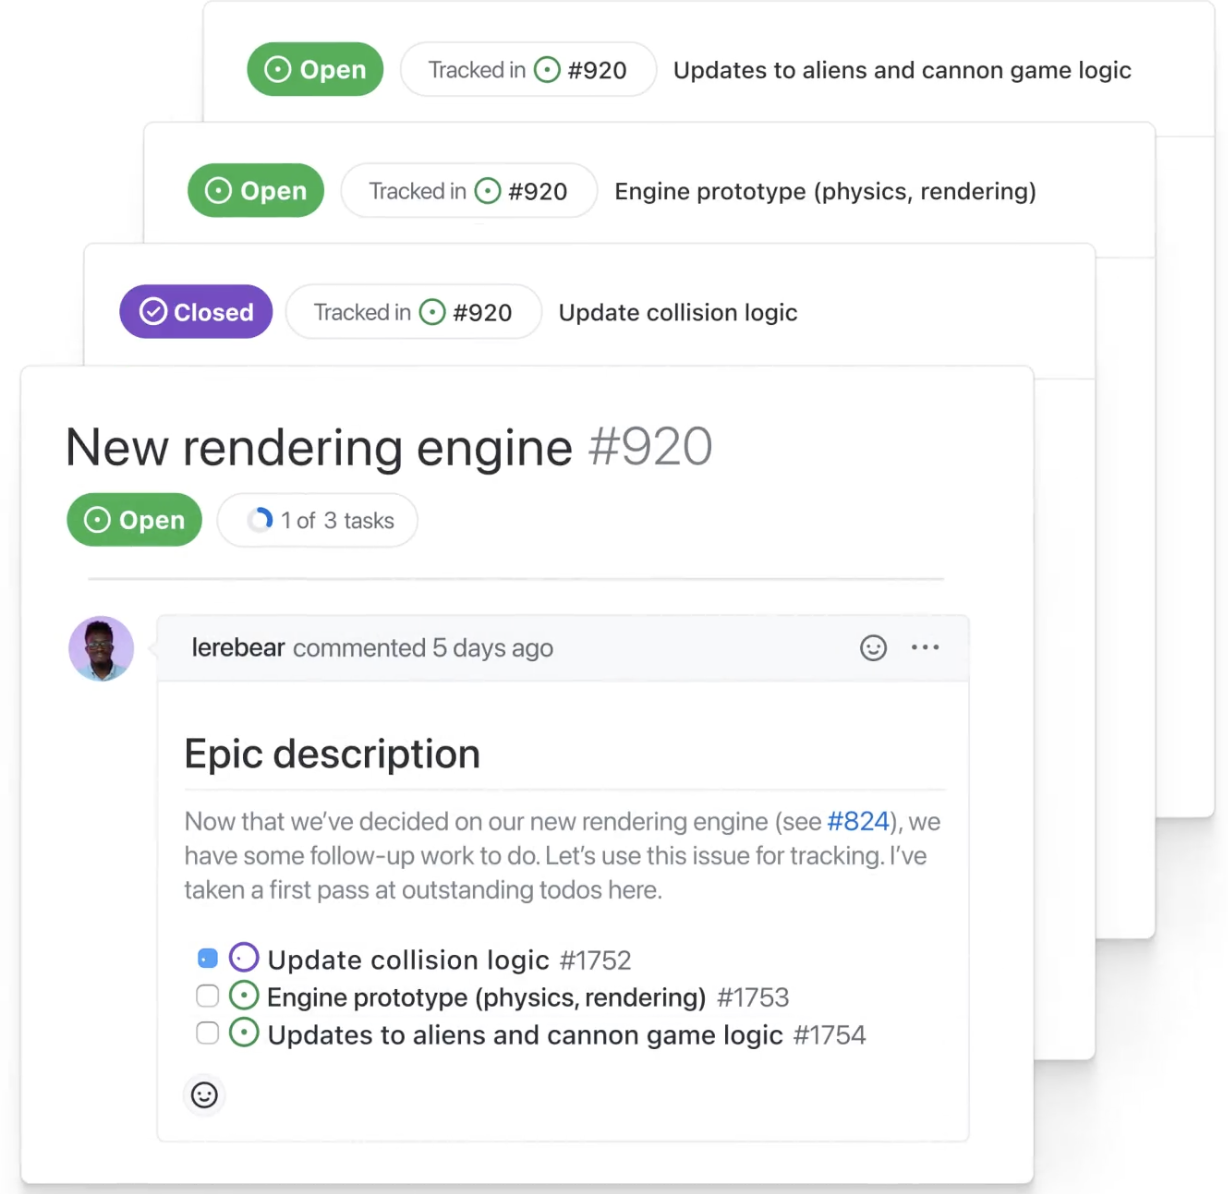
\includegraphics[width=.9\linewidth]{../../figures/issues-2.png}}
    \only<3>{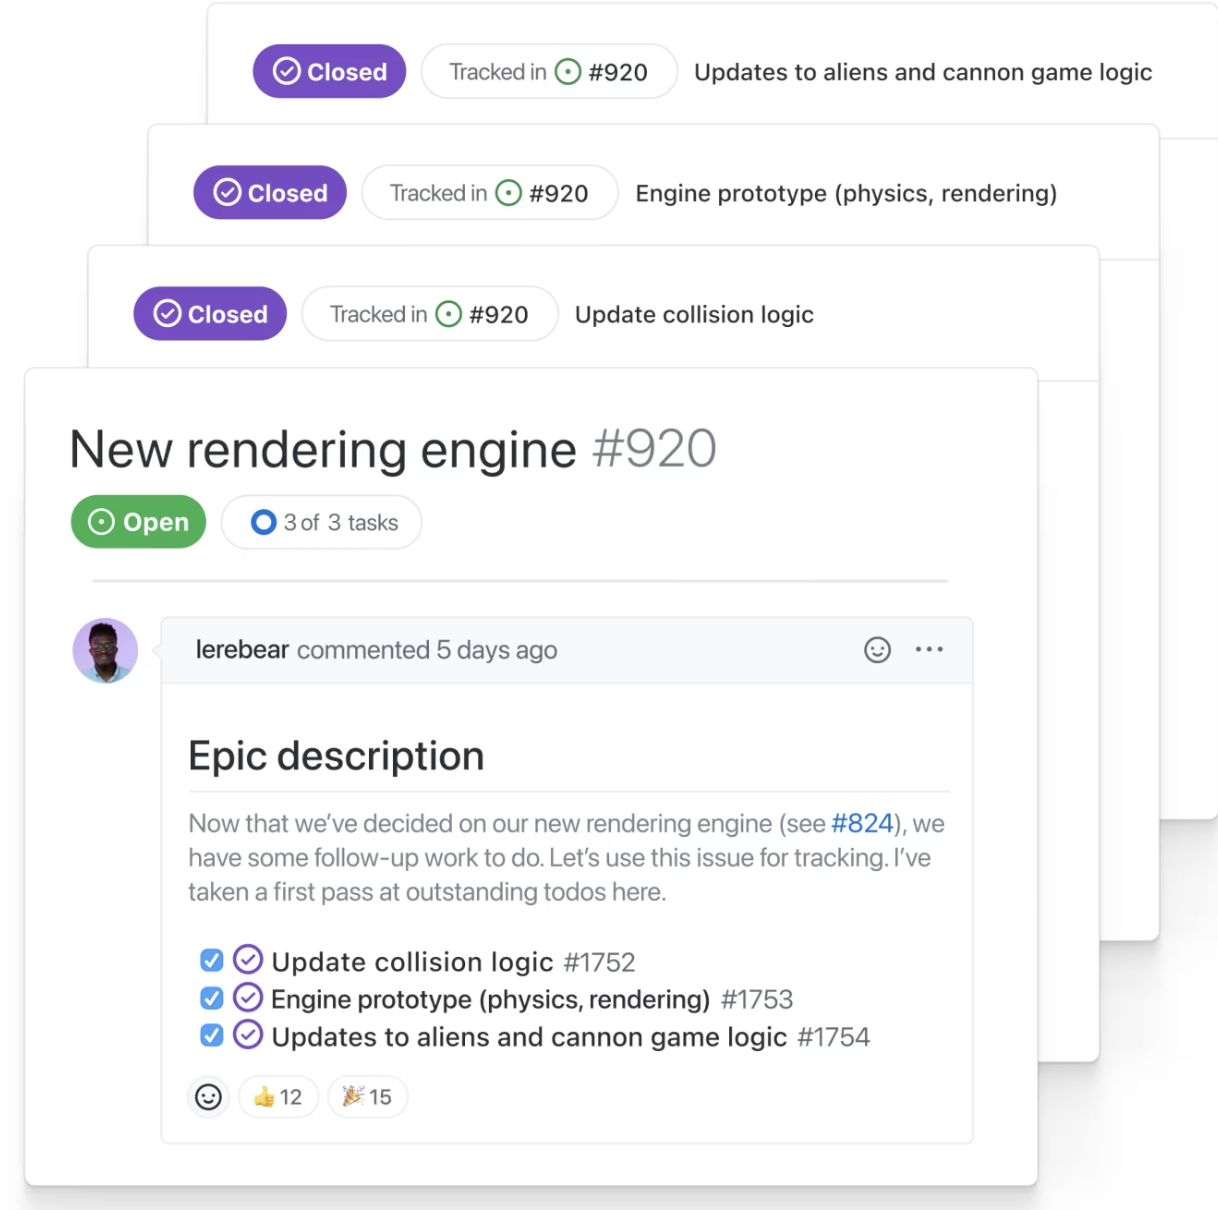
\includegraphics[width=.9\linewidth]{../../figures/issues-3.png}}
  \end{columns}
\end{frame}


\section{Conversations}

\begin{frame}
  \frametitle{\insertsectionhead}
  \framesubtitle{\insertsubsectionhead}
  \begin{columns}
    \column{.45\textwidth}
    \scriptsize
    \begin{itemize}
      \item Move conversations forward
      \item Express ideas with GitHub Flavored Markdown, 
      \item mention contributors, 
      \item react with emoji, 
      \item clarify with attachments(videos, pdf, images...), 
      \item see references from commits, pull requests, releases, and deploys. 
      \item Coordinate by assigning contributors and teams, 
      \item or by adding them to milestones and projects. 
    \end{itemize}
    \centering\vspace{1cm}
    \alert{All in a single timeline.}
    \column{.45\textwidth}
    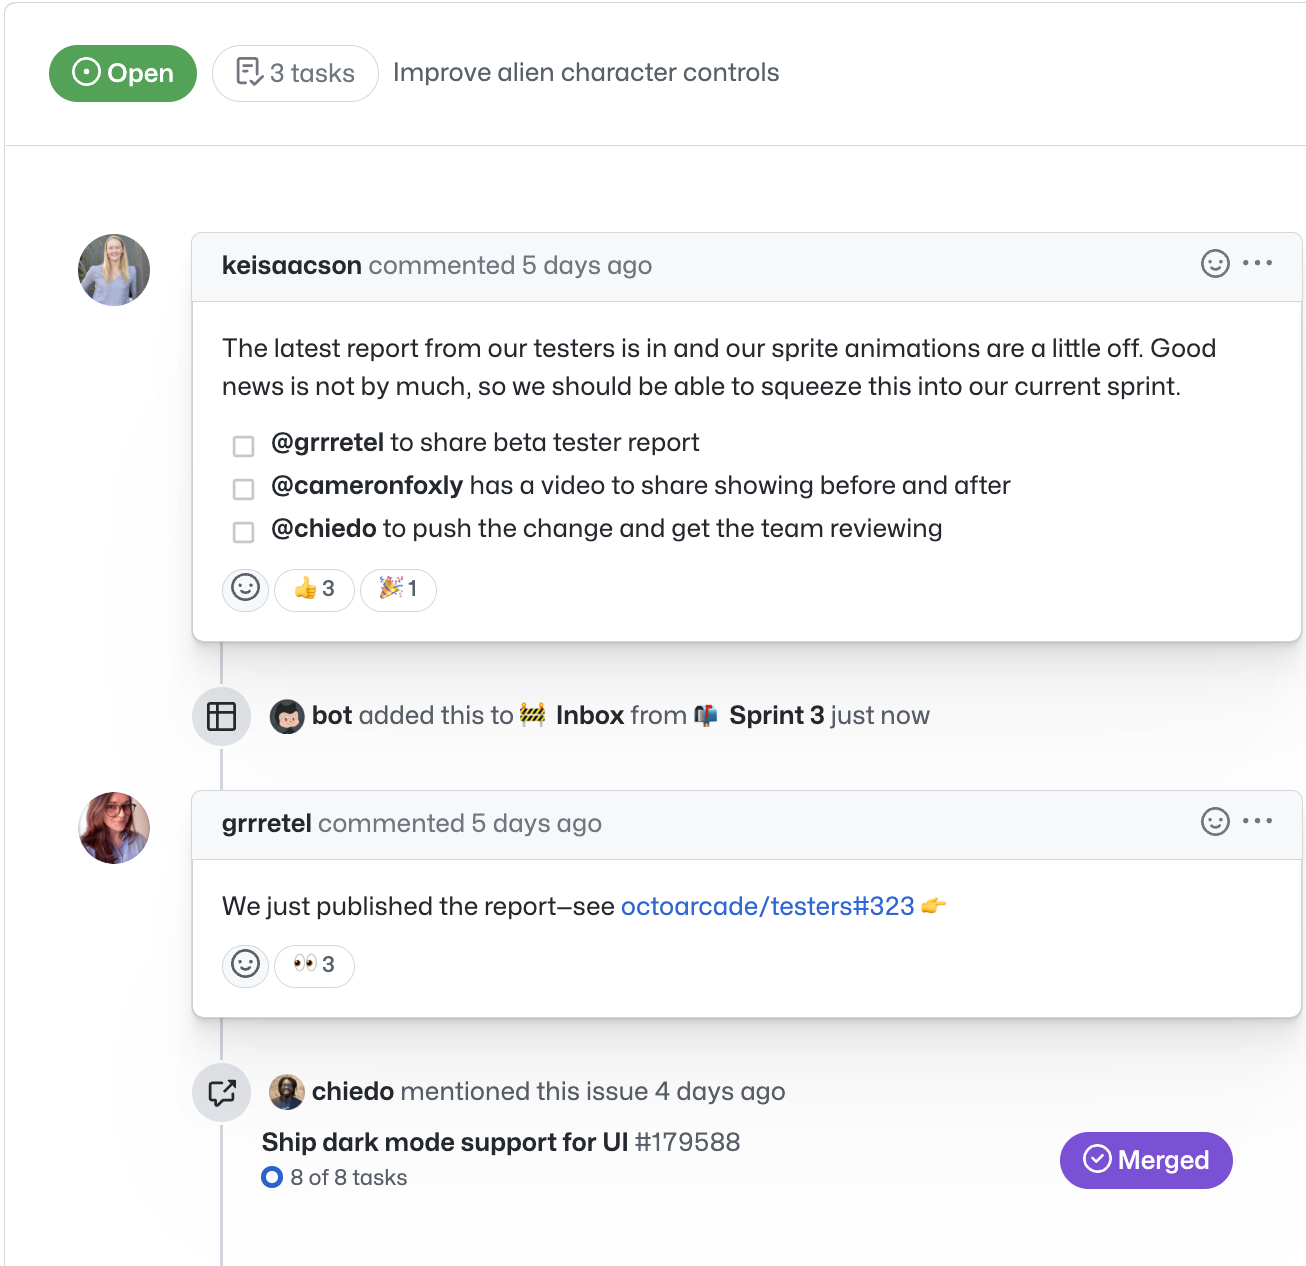
\includegraphics[width=.9\linewidth]{../../figures/conversations-1.png}
  \end{columns}

\end{frame}

\section{Create views}
\begin{frame}
  \frametitle{\insertsectionhead}
  \framesubtitle{\insertsubsectionhead}
  \begin{columns}
    \column{.4\textwidth}
    \begin{itemize}
      \item Save views for sprints, backlogs, teams, or releases. 
      \item Rank, group, sort, and filter issues to suit the occasion. 
      \item Choose between tables, boards, and timelines.
    \end{itemize}
    \column{.55\textwidth}
    \only<1>{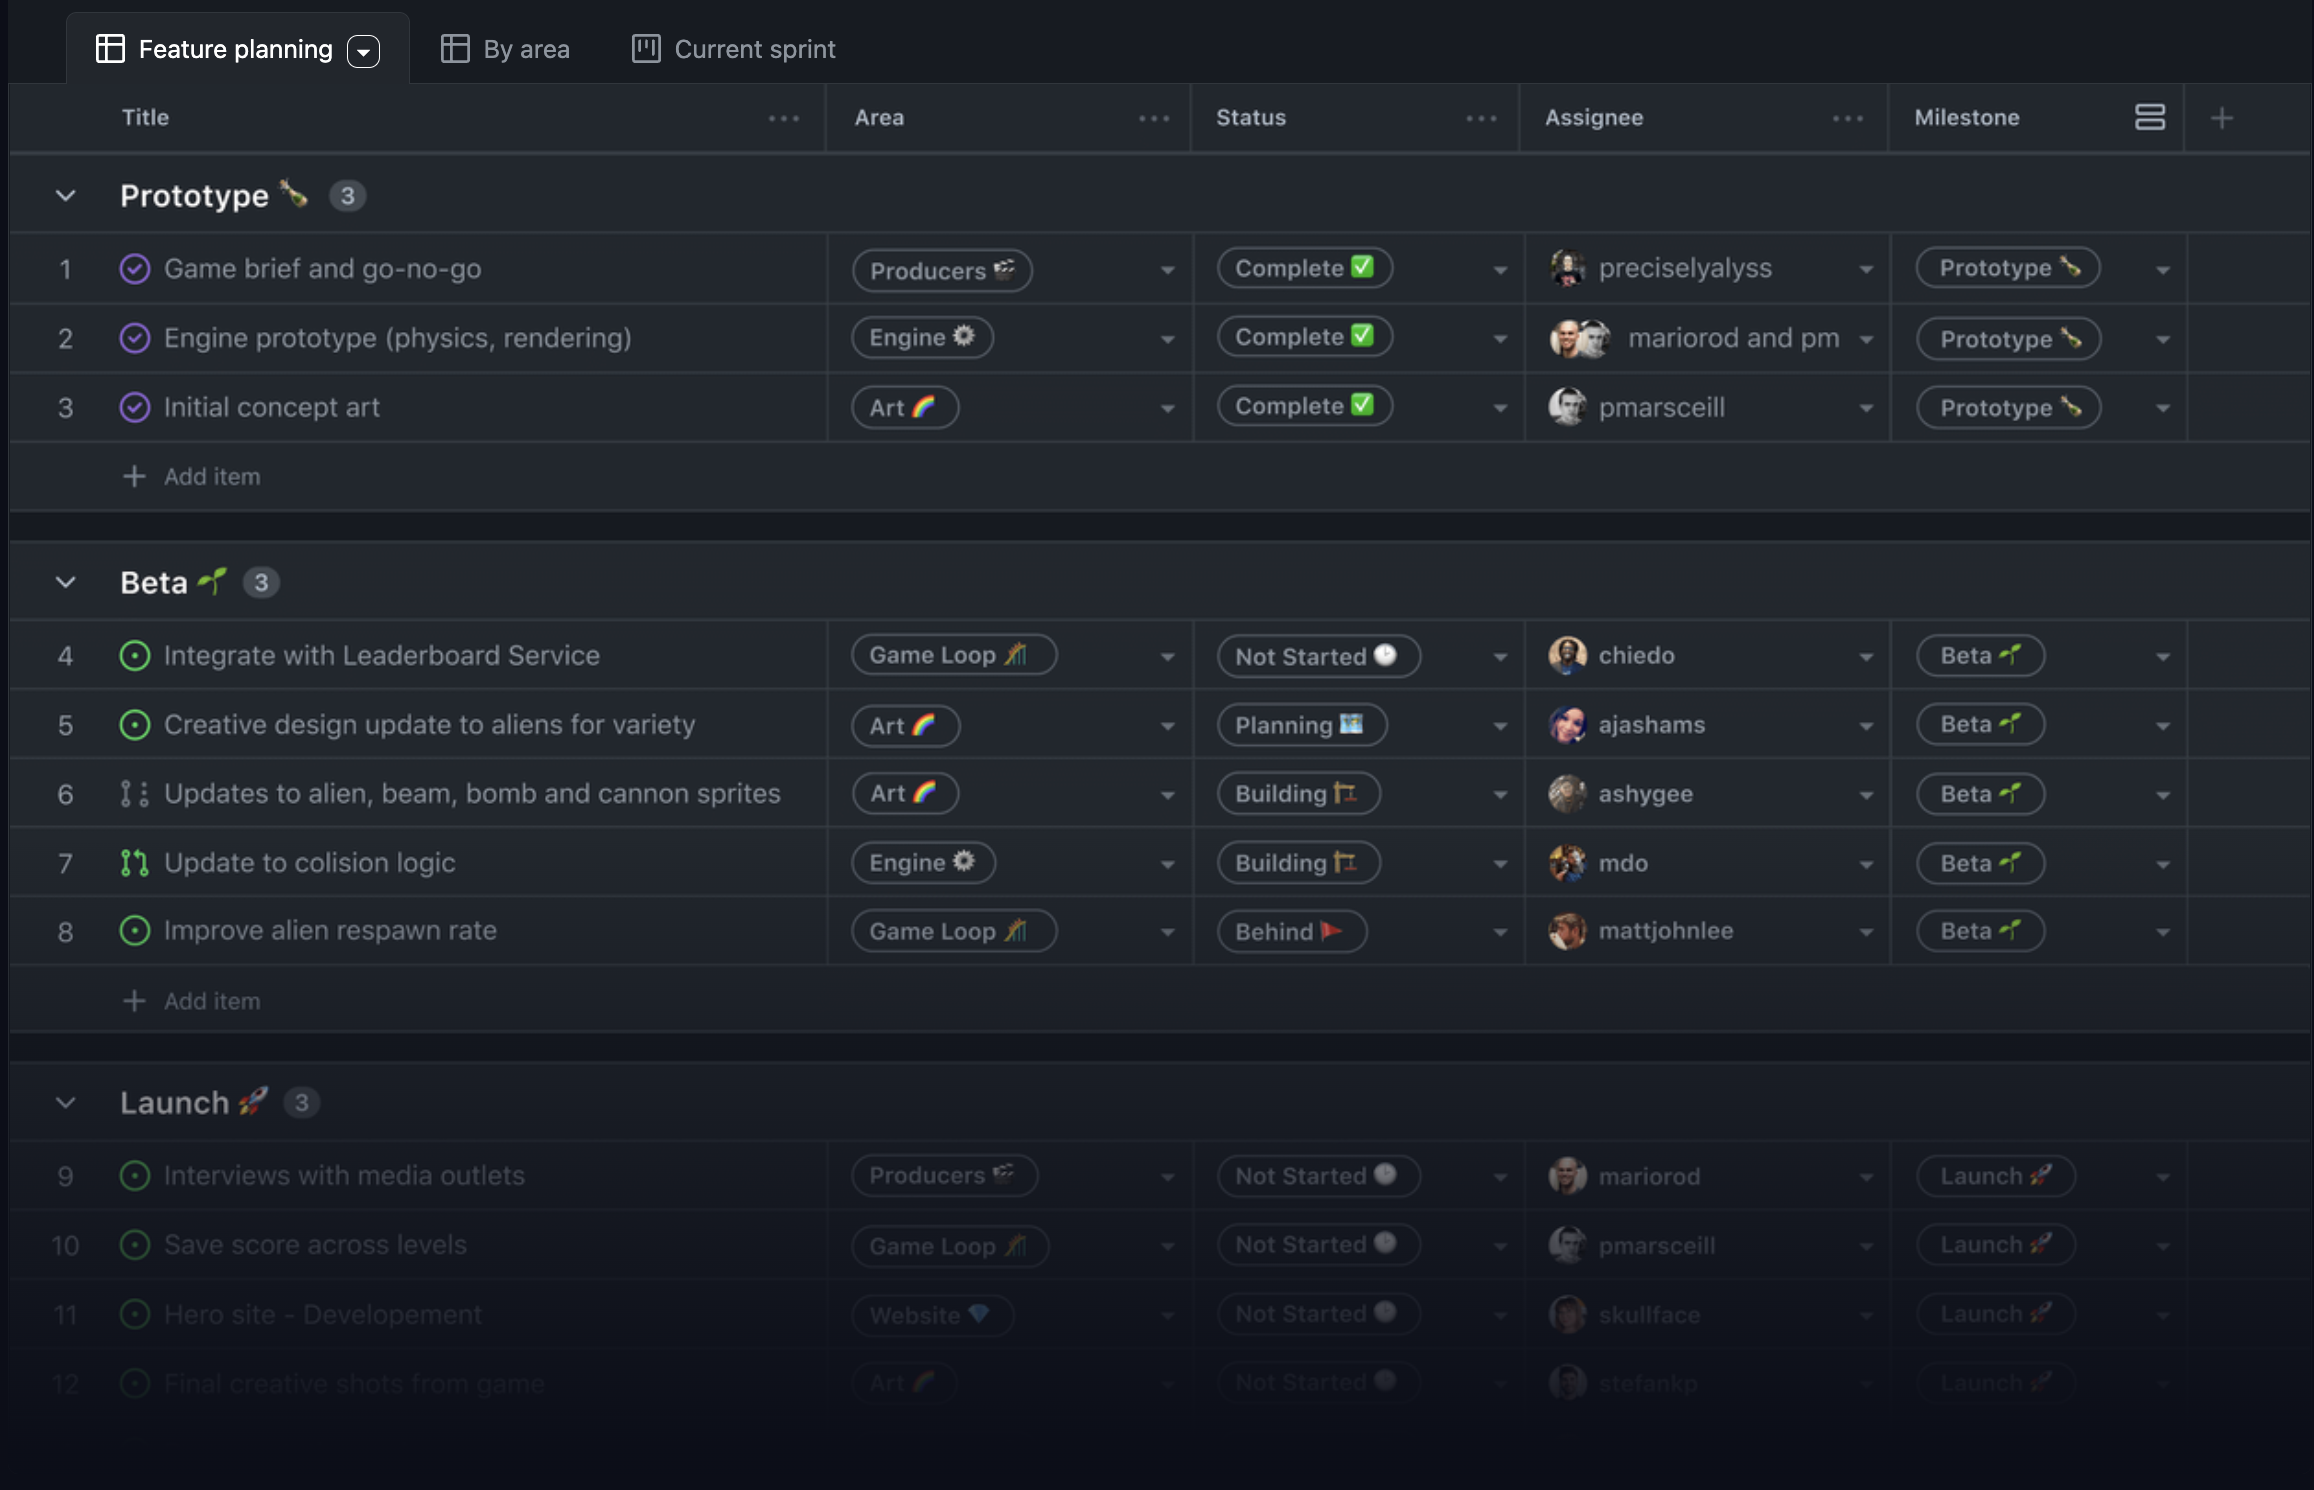
\includegraphics[width=.95\linewidth]{../../figures/views-1.png}}
    \only<2>{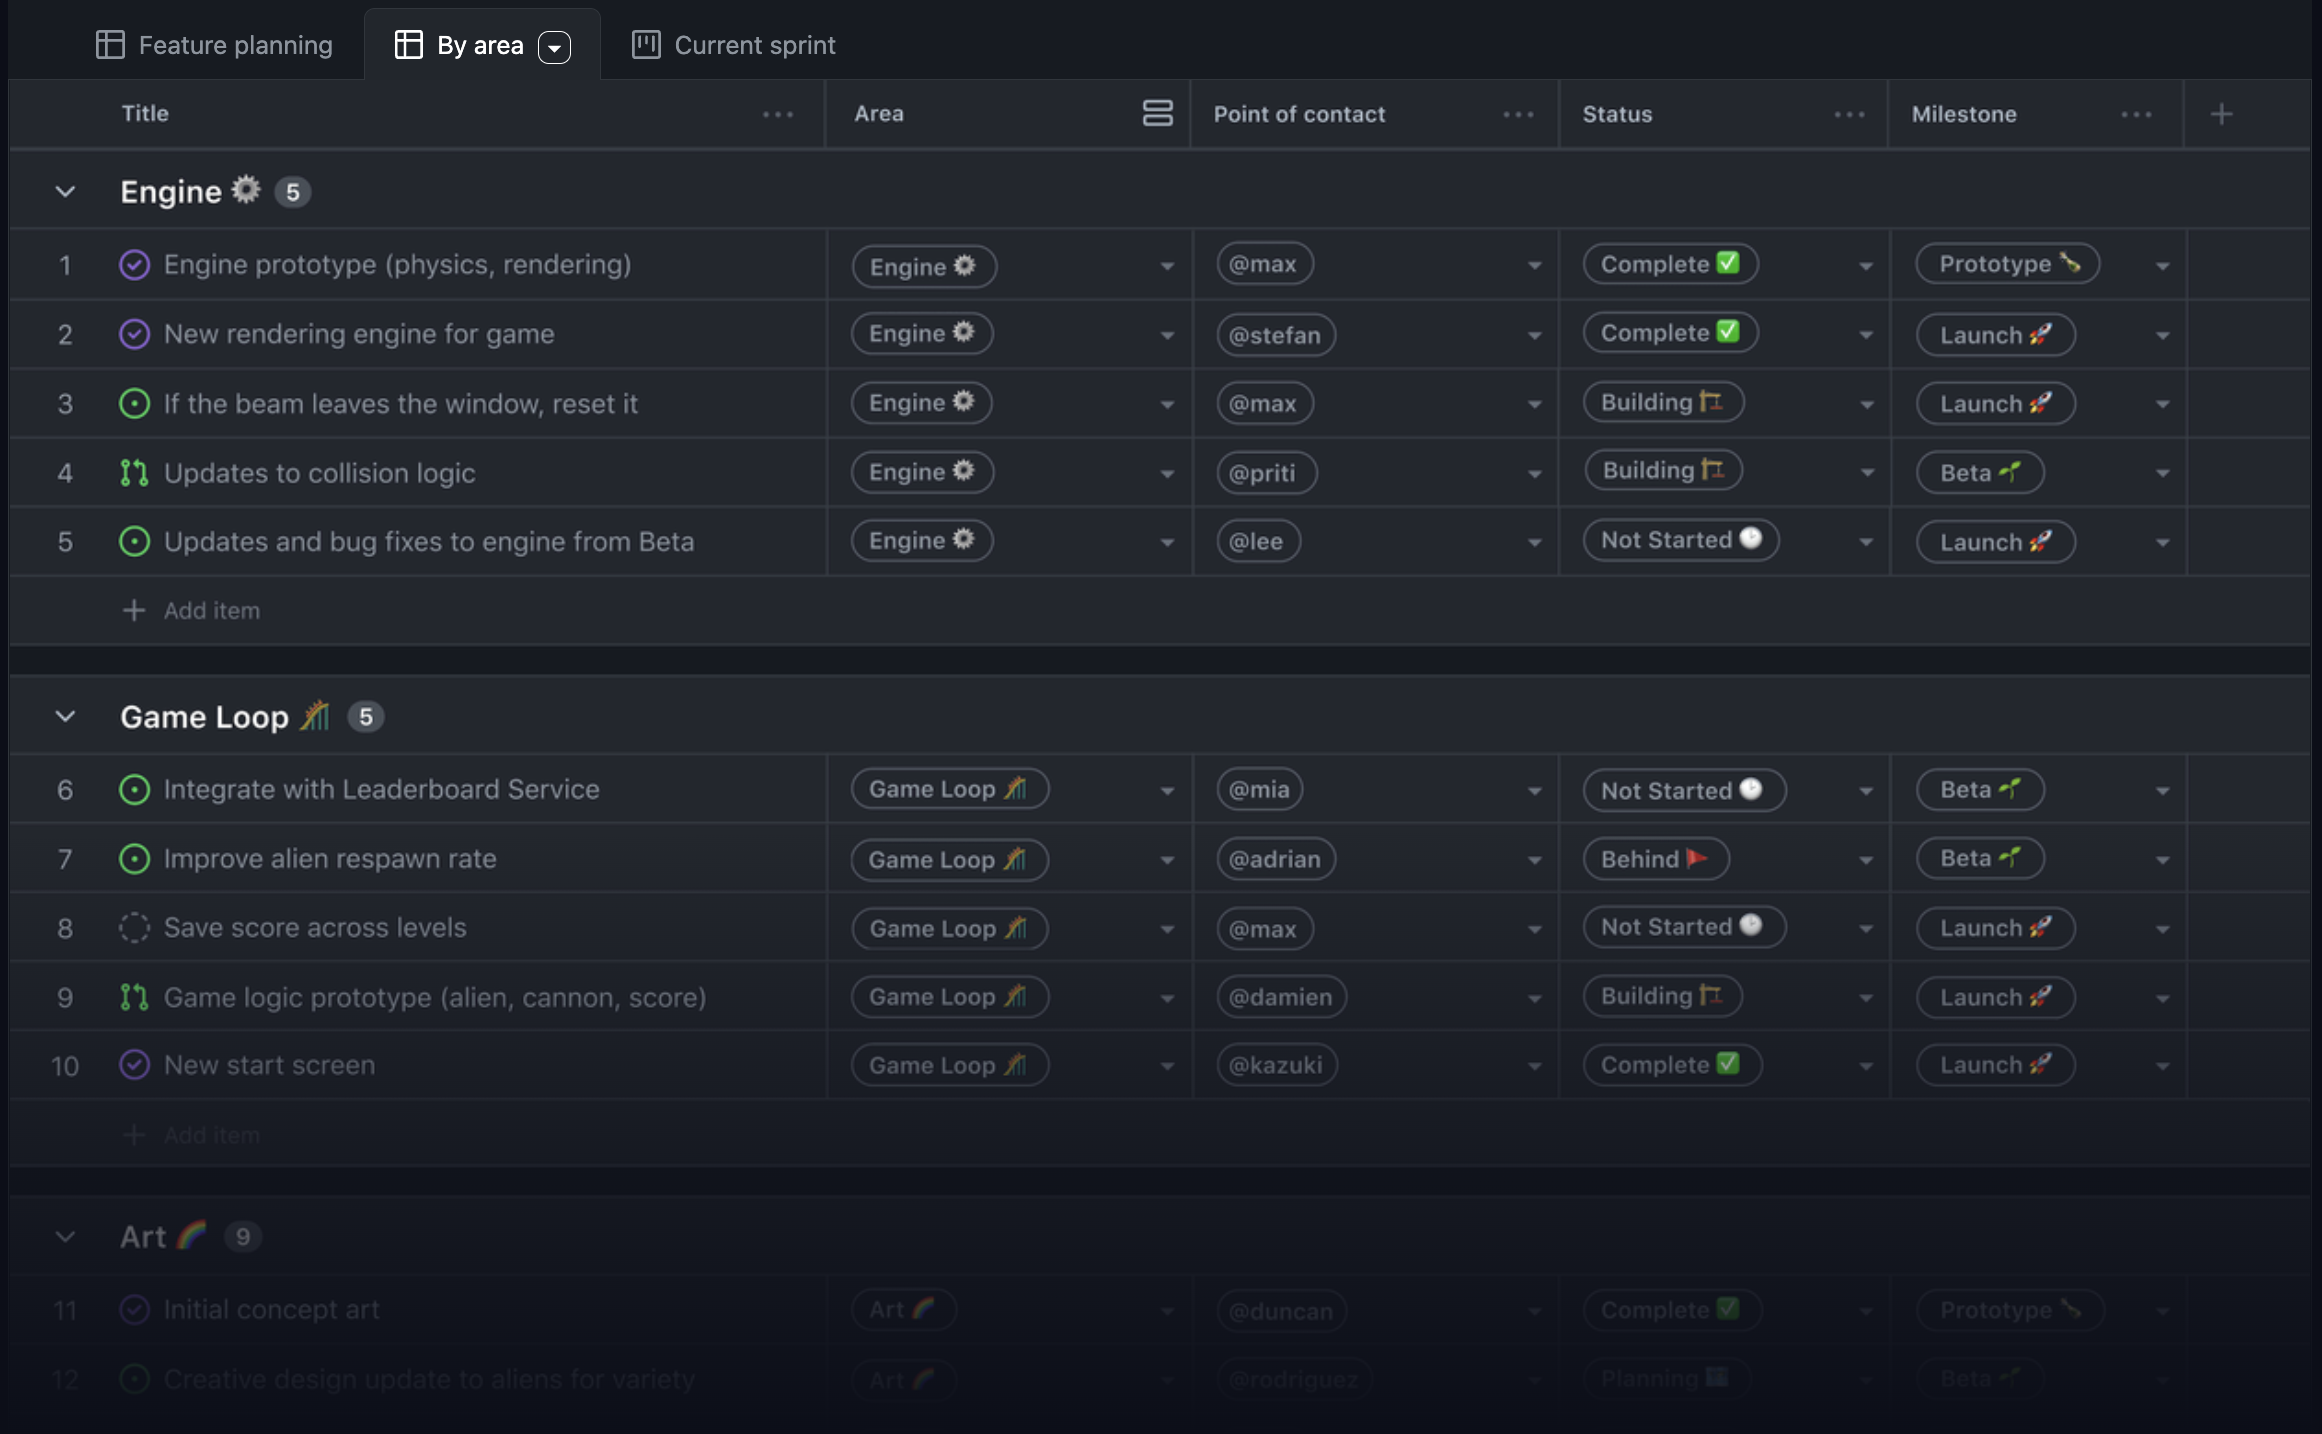
\includegraphics[width=.95\linewidth]{../../figures/views-2.png}}
    \only<3>{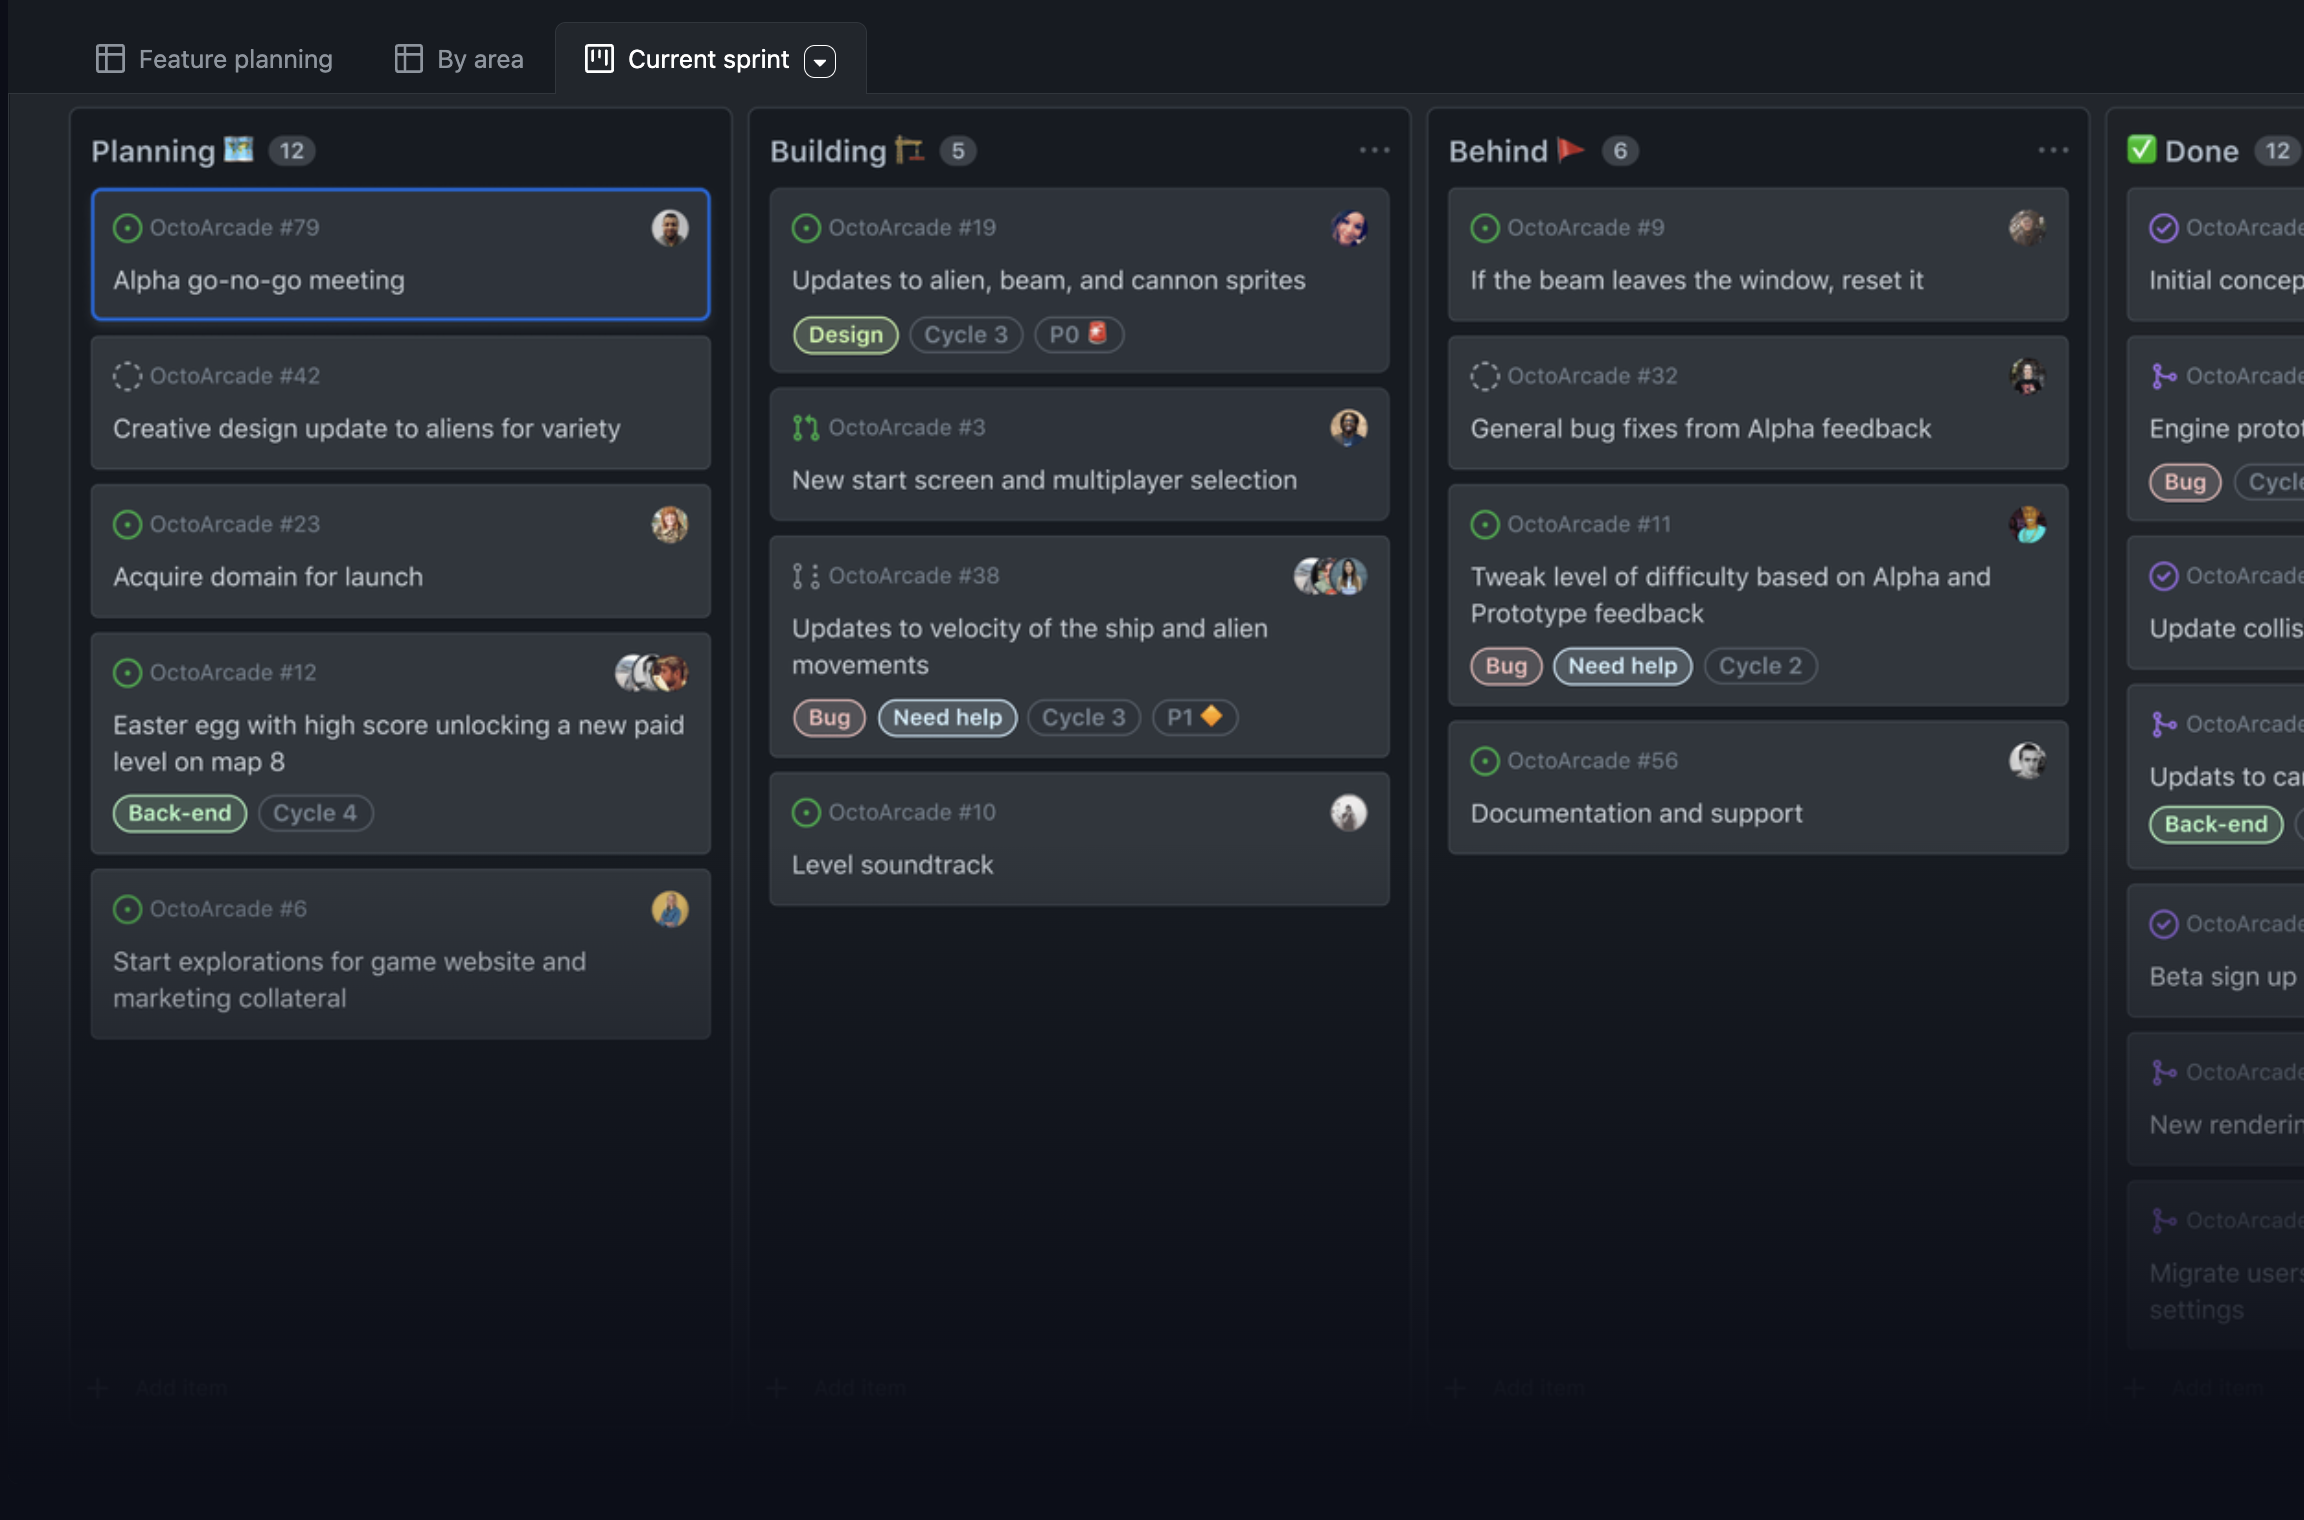
\includegraphics[width=.95\linewidth]{../../figures/views-3.png}}
  \end{columns}

\end{frame}

\section{Extend issues with custom fields}

\begin{frame}
  \frametitle{\insertsectionhead}
  \framesubtitle{\insertsubsectionhead}
  \begin{columns}
    \column{.4\textwidth}
    \begin{itemize}
      \item Track metadata like iterations, priority, story points, dates, notes, and links. 
      \item Add custom fields to project tables 
      \item edit from the issue sidebar.
    \end{itemize}
    \column{.55\textwidth}
    \only<1>{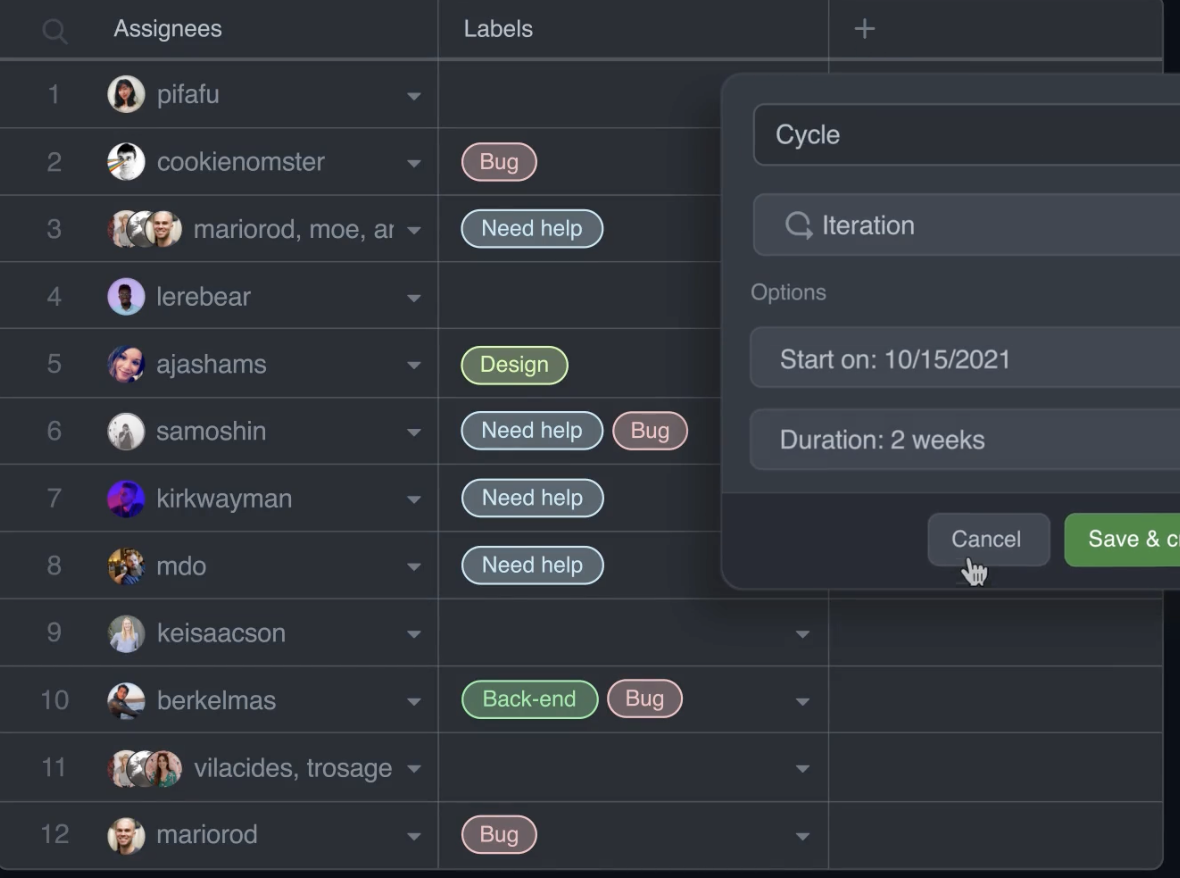
\includegraphics[width=.95\linewidth]{../../figures/custom-fields-1.png}}
    \only<2>{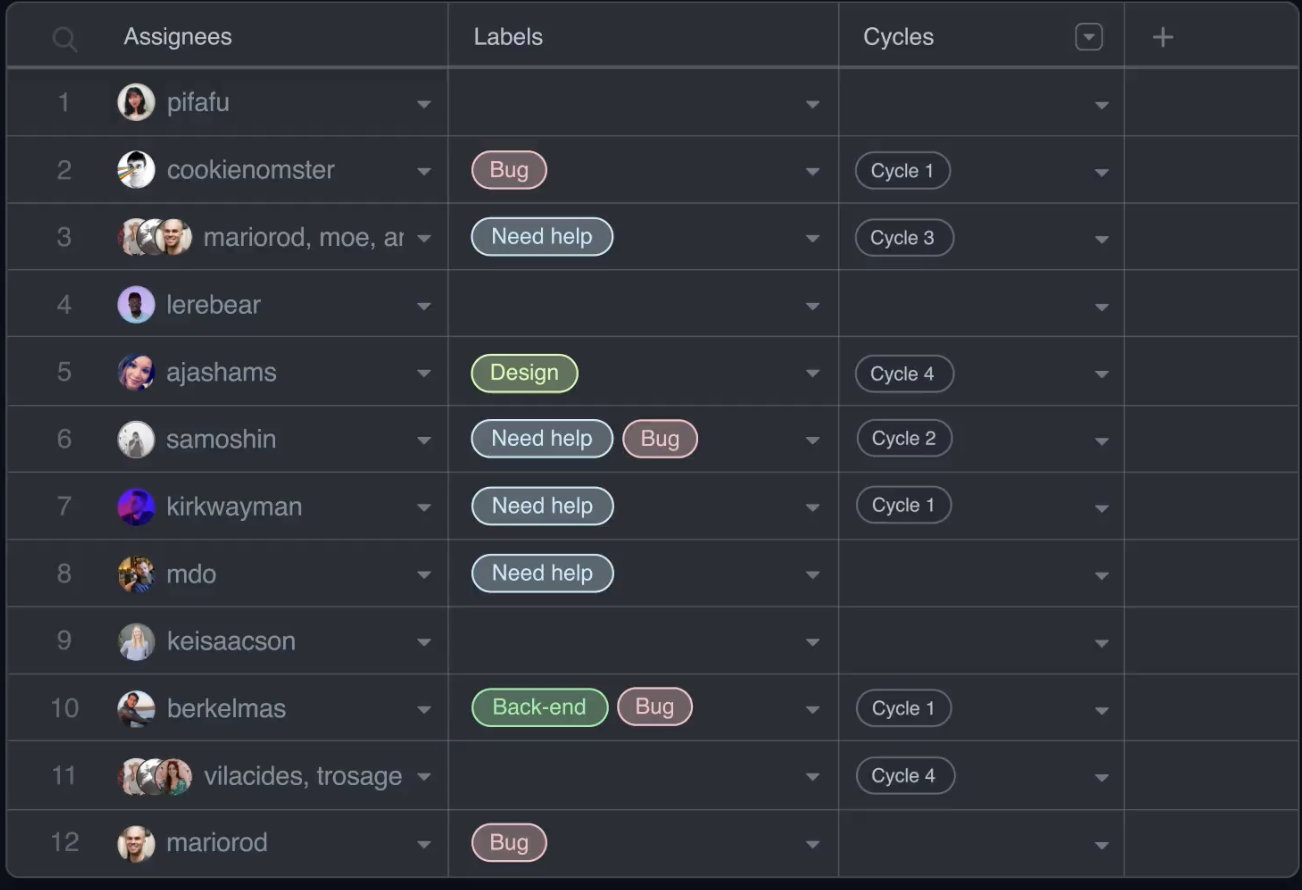
\includegraphics[width=.95\linewidth]{../../figures/custom-fields-2.png}}
  \end{columns}
  

\end{frame}
\begin{frame}
  \frametitle{\insertsectionhead}
  \framesubtitle{\insertsubsectionhead}

  \begin{columns}
    \column{.4\textwidth}
    \begin{itemize}
      \item Track the health of your current iteration cycle, milestone, or any other custom field you create with new project insights.
      \item  Identify bottlenecks and issues blocking the team from making progress with the burn up charts.
    \end{itemize}
    \column{.55\textwidth}
    \only<1>{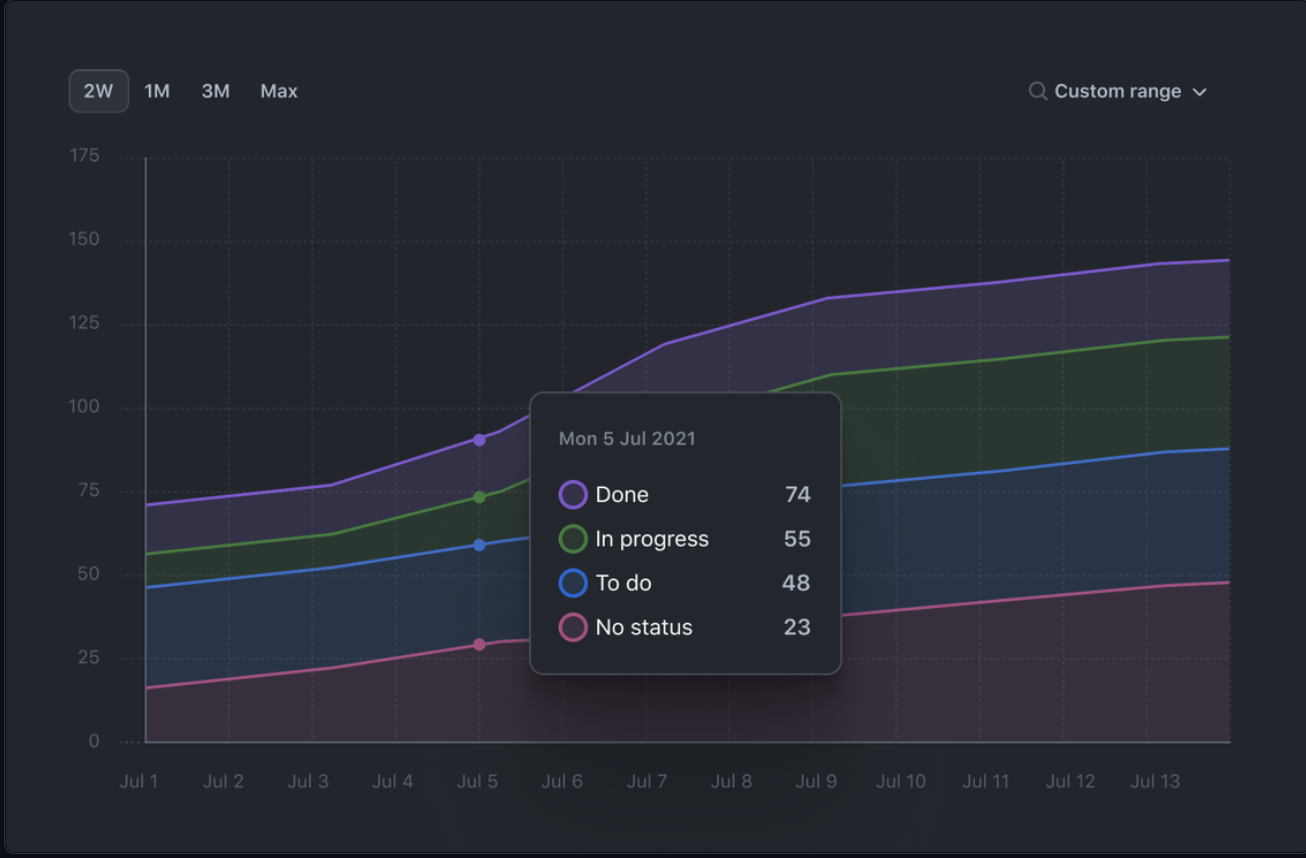
\includegraphics[width=.95\linewidth]{../../figures/charts-1.png}}
  \end{columns}


\end{frame}
\section*{Automate workflows}
\begin{frame}
  \frametitle{\insertsectionhead}
  \framesubtitle{\insertsubsectionhead}
  \begin{columns}
    \column{.4\textwidth}
    \begin{itemize}
      \item  Automate the project planning with workflows. 
      \item Automatically triage issues, set values for custom fields, react to changes, or schedule something. 
      \item You can even tee them up to run an Action.
    \end{itemize}
    \column{.55\textwidth}
    \only<1>{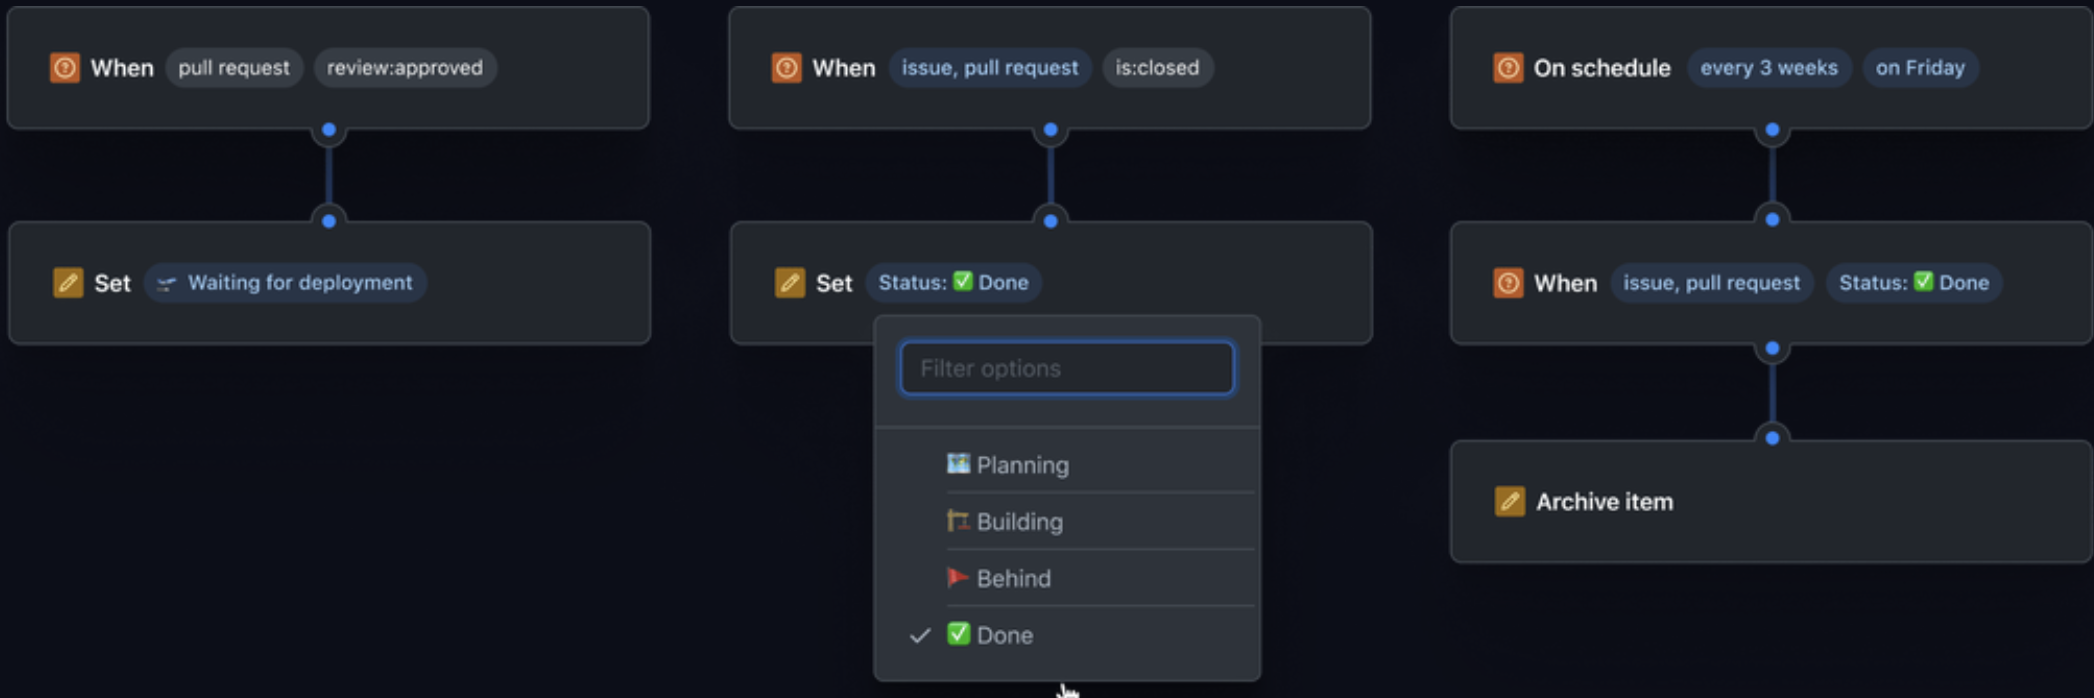
\includegraphics[width=.95\linewidth]{../../figures/workfflows-1.png}}
  \end{columns}

\end{frame}


\end{document}